\documentclass[10pt,a4paper]{article}

% --- Pakiety ---------------------------------------------------------------
\usepackage{iftex}
\ifXeTeX
  \usepackage{fontspec} % XeTeX/Tectonic: czcionki Unicode (domyślnie Latin Modern)
\else
  \usepackage[utf8]{inputenc}
  \usepackage[T1]{fontenc}
  \usepackage{lmodern}
\fi
\usepackage[polish]{babel}
\usepackage{xcolor}
\usepackage[margin=1.9cm]{geometry}
\usepackage{amsmath,amssymb,mathtools}
\usepackage{graphicx}
\usepackage{booktabs}
\usepackage{listings}
\usepackage{algorithm}
\usepackage{algpseudocode}
\usepackage[font=small,labelfont=bf,skip=3pt]{caption}
\usepackage{enumitem}
\usepackage{microtype}

\setlist{itemsep=1pt,topsep=2pt,parsep=0pt}
\setlength{\parindent}{0pt}
\setlength{\parskip}{3pt}
\renewcommand{\arraystretch}{1.1}

% Styl fragmentów kodu C++
\lstset{
  language=C++,
  basicstyle=\ttfamily\scriptsize,
  keywordstyle=\bfseries,
  commentstyle=\itshape\color[gray]{0.35},
  numbers=left, numberstyle=\tiny, numbersep=4pt,
  frame=single, framerule=0.3pt, rulecolor=\color[gray]{0.6},
  xleftmargin=10pt, aboveskip=3pt, belowskip=3pt,
  columns=fullflexible, keepspaces=true, showstringspaces=false
}

% Pseudokod: polskie słowa kluczowe
\floatname{algorithm}{Algorytm}
\algrenewcommand\algorithmicrequire{\textbf{Wejście:}}
\algrenewcommand\algorithmicensure{\textbf{Wyjście:}}
\algrenewcommand\algorithmicif{\textbf{jeżeli}}
\algrenewcommand\algorithmicthen{\textbf{to}}
\algrenewcommand\algorithmicelse{\textbf{w przeciwnym razie}}
\algrenewcommand\algorithmicreturn{\textbf{zwróć}}
\algrenewtext{EndIf}{\textbf{koniec jeżeli}}
\algrenewtext{If}[1]{\textbf{jeżeli} #1 \textbf{to}}
\algrenewtext{ElsIf}[1]{\textbf{w przeciwnym razie, jeżeli} #1 \textbf{to}}
\algrenewtext{Else}{\textbf{w przeciwnym razie}}
\algrenewtext{Return}{\textbf{zwróć}}

\title{\vspace{-1.2cm}\textbf{Rekurencyjne mnożenie macierzy:\\ metody Binét'a, Strassena i Ladermana}\vspace{-0.3cm}}
\author{Imię Nazwisko (nr albumu) \quad\textbullet\quad Imię Nazwisko (nr albumu)}
\date{\today}

\begin{document}
\maketitle
\vspace{-0.6cm}

\section{Cel i zakres}
Zaimplementowano w C++ trzy rekurencyjne algorytmy mnożenia macierzy kwadratowych
o \emph{dowolnym} rozmiarze $n\times n$ (nie tylko będącym potęgą dwójki lub trójki): metodę Binét'a (podział
na $2\times2$ bloki, 8 mnożeń bloków), metodę Strassena ($2\times2$ bloki, 7 mnożeń) i metodę Ladermana
($3\times3$ bloki, 23 mnożenia zamiast 27). Macierze zawierają liczby losowe z rozkładu równomiernego
na przedziale $[10^{-8}, 1)$. Zliczano liczbę operacji zmiennoprzecinkowych $(+,-,*,/)$ oraz mierzono czas
działania. Źródła: \texttt{binet.cpp}, \texttt{strassen.cpp}, \texttt{laderman.cpp}; skrypty raportowe:
\texttt{make\_plots.py}, \texttt{compare.m}.

\section{Pseudokod algorytmów rekurencyjnych}
W metodach Binét'a i Strassena macierze dzielimy na cztery bloki $A=\begin{psmallmatrix}A_{11}&A_{12}\\A_{21}&A_{22}\end{psmallmatrix}$,
analogicznie $B$ i $C=AB$.

\begin{minipage}[t]{0.495\textwidth}
\begin{algorithm}[H]
\caption{\textsc{Binét}$(A,B)$ (\textsc{B} = wywołanie rekurencyjne)}
\begin{algorithmic}[1]
\Require $A$: $p\times q$, $B$: $q\times r$
\Ensure $C=AB$: $p\times r$
\If{$p=1$ lub $q=1$ lub $r=1$}
  \State \Return \textsc{MnożenieKlasyczne}$(A,B)$
\EndIf
\State $p_h,q_h,r_h \gets \lceil p/2\rceil,\lceil q/2\rceil,\lceil r/2\rceil$
\State podziel $A$ w punktach $(p_h,q_h)$, $B$ w $(q_h,r_h)$
\State $C_{11}\gets \textsc{B}(A_{11},B_{11})+\textsc{B}(A_{12},B_{21})$
\State $C_{12}\gets \textsc{B}(A_{11},B_{12})+\textsc{B}(A_{12},B_{22})$
\State $C_{21}\gets \textsc{B}(A_{21},B_{11})+\textsc{B}(A_{22},B_{21})$
\State $C_{22}\gets \textsc{B}(A_{21},B_{12})+\textsc{B}(A_{22},B_{22})$
\State \Return $\begin{psmallmatrix}C_{11}&C_{12}\\C_{21}&C_{22}\end{psmallmatrix}$
\end{algorithmic}
\end{algorithm}
\end{minipage}\hfill
\begin{minipage}[t]{0.495\textwidth}
\begin{algorithm}[H]
\caption{\textsc{Strassen}$(A,B)$, $n\times n$ (\textsc{S} = wywołanie rekurencyjne)}
\begin{algorithmic}[1]
\If{$n=1$} \State \Return $A\cdot B$ \EndIf
\If{$n$ nieparzyste, $m=n-1$}
  \State wydziel $A_{11}$ ($m{\times}m$), kolumnę $a_{12}$, wiersz $a_{21}$, liczbę $a_{22}$ (tak samo $B$)
  \State $C_{11}\gets \textsc{S}(A_{11},B_{11})+a_{12}b_{21}$
  \State $C_{12}\gets A_{11}b_{12}+a_{12}b_{22}$
  \State $C_{21}\gets a_{21}B_{11}+a_{22}b_{21}$
  \State $C_{22}\gets a_{21}b_{12}+a_{22}b_{22}$
\Else
  \State $M_1\gets \textsc{S}(A_{11}{+}A_{22},\,B_{11}{+}B_{22})$
  \State $M_2\gets \textsc{S}(A_{21}{+}A_{22},\,B_{11})$
  \State $M_3\gets \textsc{S}(A_{11},\,B_{12}{-}B_{22})$
  \State $M_4\gets \textsc{S}(A_{22},\,B_{21}{-}B_{11})$
  \State $M_5\gets \textsc{S}(A_{11}{+}A_{12},\,B_{22})$
  \State $M_6\gets \textsc{S}(A_{21}{-}A_{11},\,B_{11}{+}B_{12})$
  \State $M_7\gets \textsc{S}(A_{12}{-}A_{22},\,B_{21}{+}B_{22})$
  \State $C_{11}\gets M_1{+}M_4{-}M_5{+}M_7$, \; $C_{12}\gets M_3{+}M_5$
  \State $C_{21}\gets M_2{+}M_4$, \; $C_{22}\gets M_1{-}M_2{+}M_3{+}M_6$
\EndIf
\State \Return $C$ złożone z $C_{11},C_{12},C_{21},C_{22}$
\end{algorithmic}
\end{algorithm}
\end{minipage}

W metodzie Ladermana dzielimy $A$, $B$ i $C$ na $3\times3$ bloki $A_{ij}$, $B_{ij}$, $C_{ij}$ ($i,j=1,2,3$)
o rozmiarze $h=n/3$. Zamiast 27 iloczynów bloków (jak w podejściu klasycznym) wystarczą 23:
{\small
\begin{equation}\label{eq:laderman-m}
\begin{aligned}
M_{1}  &= (A_{11}{+}A_{12}{+}A_{13}{-}A_{21}{-}A_{22}{-}A_{32}{-}A_{33})\,B_{22} &
M_{2}  &= (A_{11}{-}A_{21})(B_{22}{-}B_{12}) \\
M_{3}  &= A_{22}\,(B_{12}{+}B_{21}{+}B_{33}{-}B_{11}{-}B_{22}{-}B_{23}{-}B_{31}) &
M_{4}  &= (A_{21}{+}A_{22}{-}A_{11})(B_{11}{+}B_{22}{-}B_{12}) \\
M_{5}  &= (A_{21}{+}A_{22})(B_{12}{-}B_{11}) &
M_{6}  &= A_{11}B_{11} \\
M_{7}  &= (A_{31}{+}A_{32}{-}A_{11})(B_{11}{+}B_{23}{-}B_{13}) &
M_{8}  &= (A_{31}{-}A_{11})(B_{13}{-}B_{23}) \\
M_{9}  &= (A_{31}{+}A_{32})(B_{13}{-}B_{11}) &
M_{10} &= (A_{11}{+}A_{12}{+}A_{13}{-}A_{22}{-}A_{23}{-}A_{31}{-}A_{32})\,B_{23} \\
M_{11} &= A_{32}\,(B_{13}{+}B_{21}{+}B_{32}{-}B_{11}{-}B_{22}{-}B_{23}{-}B_{31}) &
M_{12} &= (A_{32}{+}A_{33}{-}A_{13})(B_{22}{+}B_{31}{-}B_{32}) \\
M_{13} &= (A_{13}{-}A_{33})(B_{22}{-}B_{32}) &
M_{14} &= A_{13}B_{31} \\
M_{15} &= (A_{32}{+}A_{33})(B_{32}{-}B_{31}) &
M_{16} &= (A_{22}{+}A_{23}{-}A_{13})(B_{23}{+}B_{31}{-}B_{33}) \\
M_{17} &= (A_{13}{-}A_{23})(B_{23}{-}B_{33}) &
M_{18} &= (A_{22}{+}A_{23})(B_{33}{-}B_{31}) \\
M_{19} &= A_{12}B_{21},\quad M_{20} = A_{23}B_{32},\quad M_{21} = A_{21}B_{13} &
M_{22} &= A_{31}B_{12},\quad M_{23} = A_{33}B_{33}
\end{aligned}
\end{equation}
\begin{equation}\label{eq:laderman-c}
\begin{aligned}
C_{11} &= M_6{+}M_{14}{+}M_{19} &
C_{12} &= M_1{+}M_4{+}M_5{+}M_6{+}M_{12}{+}M_{14}{+}M_{15} \\
C_{13} &= M_6{+}M_7{+}M_9{+}M_{10}{+}M_{14}{+}M_{16}{+}M_{18} &
C_{21} &= M_2{+}M_3{+}M_4{+}M_6{+}M_{14}{+}M_{16}{+}M_{17} \\
C_{22} &= M_2{+}M_4{+}M_5{+}M_6{+}M_{20} &
C_{23} &= M_{14}{+}M_{16}{+}M_{17}{+}M_{18}{+}M_{21} \\
C_{31} &= M_6{+}M_7{+}M_8{+}M_{11}{+}M_{12}{+}M_{13}{+}M_{14} &
C_{32} &= M_{12}{+}M_{13}{+}M_{14}{+}M_{15}{+}M_{22} \\
C_{33} &= M_6{+}M_7{+}M_8{+}M_9{+}M_{23}
\end{aligned}
\end{equation}
}%
Na jednym poziomie rekurencji są więc 23 mnożenia bloków oraz $56+42=98$ dodawań/odejmowań bloków
(w każdej sumie pierwszy składnik jest dodatni, więc nie ma osobnej operacji negacji).

\begin{algorithm}[H]
\caption{\textsc{Laderman}$(A,B)$, $n\times n$ (\textsc{L} = wywołanie rekurencyjne)}
\begin{algorithmic}[1]
\If{$n\le2$} \State \Return \textsc{MnożenieKlasyczne}$(A,B)$ \Comment{$2\times2$ nie da się podzielić na $3\times3$ bloki}
\EndIf
\State $r\gets n \bmod 3$
\If{$r\ne0$, $m=n-r$}
  \State wydziel $A_{11}$ ($m{\times}m$), paski $a_{12}$ ($m{\times}r$), $a_{21}$ ($r{\times}m$), blok $a_{22}$ ($r{\times}r$) (tak samo $B$)
  \State $C_{11}\gets \textsc{L}(A_{11},B_{11})+a_{12}b_{21}$, \; $C_{12}\gets A_{11}b_{12}+a_{12}b_{22}$
  \State $C_{21}\gets a_{21}B_{11}+a_{22}b_{21}$, \; $C_{22}\gets a_{21}b_{12}+a_{22}b_{22}$
\Else
  \State podziel $A$ i $B$ na $3\times3$ bloki o rozmiarze $h=n/3$
  \State $M_i\gets\textsc{L}(\cdot,\cdot)$ dla $i=1,\dots,23$ według \eqref{eq:laderman-m}
  \State $C_{ij}$ ze wzorów \eqref{eq:laderman-c}
\EndIf
\State \Return $C$ złożone z bloków $C_{ij}$
\end{algorithmic}
\end{algorithm}

\textbf{Dowolny rozmiar.} W metodzie Binét'a przy nieparzystych wymiarach bloki górne/lewe mają
$\lceil\cdot/2\rceil$, a dolne/prawe $\lfloor\cdot/2\rfloor$ wierszy i kolumn, więc mnożymy macierze prostokątne
(wzory na $C_{ij}$ pozostają poprawne). W metodzie Strassena dla nieparzystego $n$ „obieramy'' ostatni wiersz
i kolumnę (\emph{dynamic peeling}); rdzeń $(n{-}1)\times(n{-}1)$ mnożymy rekurencyjnie, a cienkie iloczyny
klasycznie. W metodzie Ladermana stosujemy to samo obieranie, tylko odcinamy $r=n\bmod3\in\{1,2\}$ wierszy
i kolumn, tak aby rdzeń $(n{-}r)\times(n{-}r)$ dzielił się przez 3.
Macierzy nie dopełniamy zerami, dzięki czemu liczba operacji nie jest sztucznie zawyżona.
Rekurencję prowadzimy do najmniejszych możliwych bloków (bez progu przełączenia na metodę klasyczną):
$1\times1$ u Binét'a i Strassena oraz $1\times1$ lub $2\times2$ u Ladermana.

\section{Najważniejsze fragmenty kodu}
Licznik operacji zwiększany jest tylko w dwóch miejscach: przy dodawaniu/odejmowaniu macierzy (1 operacja na element)
oraz w mnożeniu klasycznym używanym w przypadku bazowym ($pqr$ mnożeń i $pr(q{-}1)$ dodawań). U Ladermana
dodawanie wielu bloków naraz realizuje funkcja \texttt{combine} (niżej), liczona w ten sam sposób.

\begin{lstlisting}
static unsigned long long g_flops = 0;           // licznik operacji + - * /
Matrix add(const Matrix& A, const Matrix& B) {   // sub() analogicznie
    Matrix C(A.rows, A.cols);
    for (size_t k = 0; k < C.data.size(); ++k) C.data[k] = A.data[k] + B.data[k];
    g_flops += C.data.size();                    // 1 operacja na element
    return C;
}
\end{lstlisting}

\textbf{Binét} (\texttt{binet.cpp}, fragment skrócony):
\begin{lstlisting}
Matrix multiplyBinet(const Matrix& A, const Matrix& B) {
    const int p = A.rows, q = A.cols, r = B.cols;
    if (p == 1 || q == 1 || r == 1) return multiplyNaive(A, B);   // przypadek bazowy
    const int ph = (p + 1) / 2, qh = (q + 1) / 2, rh = (r + 1) / 2;  // punkty podzialu
    Matrix A11 = subMatrix(A, 0, 0, ph, qh), A12 = subMatrix(A, 0, qh, ph, q - qh);
    Matrix A21 = subMatrix(A, ph, 0, p - ph, qh), A22 = subMatrix(A, ph, qh, p - ph, q - qh);
    // ... B11, B12, B21, B22 wycinane analogicznie (wiersze wg qh, kolumny wg rh)
    Matrix C11 = add(multiplyBinet(A11, B11), multiplyBinet(A12, B21));   // 8 mnozen
    Matrix C12 = add(multiplyBinet(A11, B12), multiplyBinet(A12, B22));
    Matrix C21 = add(multiplyBinet(A21, B11), multiplyBinet(A22, B21));
    Matrix C22 = add(multiplyBinet(A21, B12), multiplyBinet(A22, B22));
    // ... sklejenie C11..C22 w macierz wynikowa p x r (placeBlock)
}
\end{lstlisting}

\textbf{Strassen} (\texttt{strassen.cpp}, fragment skrócony):
\begin{lstlisting}
Matrix multiplyStrassen(const Matrix& A, const Matrix& B) {
    const int n = A.rows;
    if (n <= STRASSEN_CUTOFF) return multiplyNaive(A, B);   // CUTOFF = 1
    if (n % 2 == 1) {                                        // obieranie: m = n-1 parzyste
        // ... A11 (m x m), a12, a21, a22 oraz b.. wycinane przez subMatrix
        Matrix C11 = add(multiplyStrassen(A11, B11), multiplyNaive(a12, b21));
        // ... C12, C21, C22: tylko "cienkie" iloczyny multiplyNaive + add
    }
    // n parzyste: 7 mnozen rekurencyjnych zamiast 8
    Matrix M1 = multiplyStrassen(add(A11, A22), add(B11, B22));
    Matrix M2 = multiplyStrassen(add(A21, A22), B11);
    Matrix M3 = multiplyStrassen(A11, sub(B12, B22));
    Matrix M4 = multiplyStrassen(A22, sub(B21, B11));
    Matrix M5 = multiplyStrassen(add(A11, A12), B22);
    Matrix M6 = multiplyStrassen(sub(A21, A11), add(B11, B12));
    Matrix M7 = multiplyStrassen(sub(A12, A22), add(B21, B22));
    Matrix C11 = add(sub(add(M1, M4), M5), M7);   Matrix C12 = add(M3, M5);
    Matrix C21 = add(M2, M4);                     Matrix C22 = add(add(sub(M1, M2), M3), M6);
    // ... sklejenie C11..C22 w macierz wynikowa n x n
}
\end{lstlisting}

\textbf{Laderman} (\texttt{laderman.cpp}, fragment skrócony). Sumy mają do 7 bloków, dlatego zamiast
zagnieżdżonych wywołań \texttt{add}/\texttt{sub} funkcja \texttt{combine} przyjmuje listę bloków dodawanych
i odejmowanych:
\begin{lstlisting}
Matrix combine(MatrixList plus, MatrixList minus = {}) {  // plus[0] + plus[1] + ... - minus[0] - ...
    auto it = plus.begin();
    Matrix C = *it;                                        // kopia pierwszego skladnika (bez operacji)
    for (++it; it != plus.end(); ++it) { /* C += *it */ g_flops += C.data.size(); }
    for (const Matrix& X : minus)      { /* C -= X   */ g_flops += C.data.size(); }
    return C;
}
Matrix multiplyLaderman(const Matrix& A, const Matrix& B) {
    const int n = A.rows;
    if (n <= LADERMAN_CUTOFF) return multiplyNaive(A, B);    // CUTOFF = 2
    const int r = n % 3;
    if (r != 0) { /* obieranie r wierszy i kolumn - jak u Strassena, rdzen m = n - r */ }
    const int h = n / 3;
    // ... A11..A33, B11..B33 wycinane przez subMatrix (bloki h x h)
    Matrix M1 = multiplyLaderman(combine({A11, A12, A13}, {A21, A22, A32, A33}), B22);
    Matrix M2 = multiplyLaderman(combine({A11}, {A21}), combine({B22}, {B12}));
    // ... M3..M23 analogicznie, wg wzorow (1)
    Matrix C11 = combine({M6, M14, M19});
    Matrix C12 = combine({M1, M4, M5, M6, M12, M14, M15});
    // ... C13..C33 wg wzorow (2), sklejenie 9 blokow w macierz n x n
}
\end{lstlisting}

\section{Środowisko pomiarowe}
\textbf{Język nie jest interpretowany:} C++ jest kompilowany z góry do natywnego kodu maszynowego ARM64
(Apple clang 21.0.0 wywoływany jako \texttt{g++}, flagi \texttt{-O2 -std=c++17}); powstały plik wykonywalny jest
uruchamiany bezpośrednio przez procesor, bez interpretera i maszyny wirtualnej. Obliczenia były jednowątkowe.
\textbf{Sprzęt:} Apple M1 Pro (8 rdzeni: 6 wydajnych + 2 energooszczędne), pamięć RAM 16~GB (LPDDR5),
system macOS 26.5. Czas mierzono zegarem \texttt{std::chrono::steady\_clock}
tylko dla samego mnożenia (bez generowania macierzy i weryfikacji): dla $n\le200$ jako minimum z 3~powtórzeń,
dla $n>200$ jako pojedynczy pomiar. Wszystkie trzy programy uruchamiano kolejno, na tym samym komputerze, więc ich
czasy są ze sobą porównywalne. Pomiary czasu wykonano dla $n=1,2,\dots,200$ oraz $n=250,300,\dots,1000$ (krok 50);
liczbę operacji wyznaczono dla \emph{każdego} $n=1,\dots,1000$, korzystając z modelu rekurencyjnego (to samo drzewo
wywołań co w algorytmie, ale bez mnożenia macierzy). Dla wszystkich zmierzonych $n$ model daje liczbę operacji
identyczną z licznikiem w działającym programie. Maksymalny rozmiar, który udało się policzyć wszystkimi trzema
metodami: $n=1000$.

\section{Wykresy}
\begin{figure}[H]
\centering
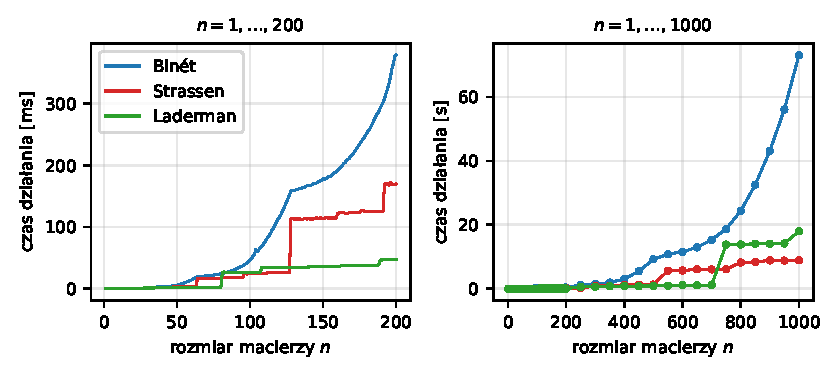
\includegraphics[width=0.86\textwidth]{data_mateusz/fig_time.pdf}
\caption{Czas działania trzech metod rekurencyjnych w zależności od rozmiaru macierzy $n$.}
\label{fig:time}
\end{figure}

\begin{figure}[H]
\centering
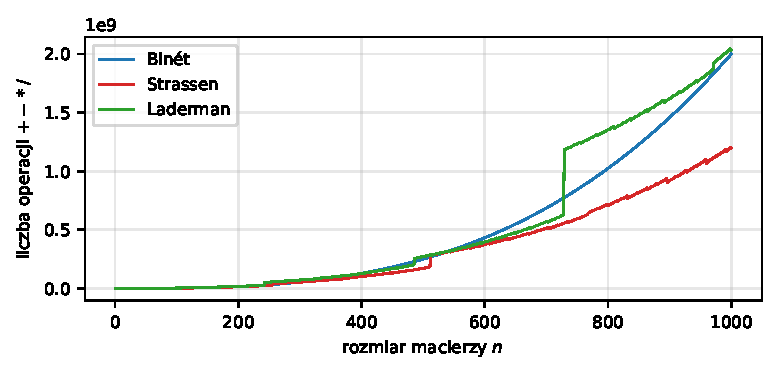
\includegraphics[width=0.78\textwidth]{data_mateusz/fig_flops.pdf}
\caption{Liczba operacji zmiennoprzecinkowych $(+,-,*,/)$ w zależności od $n$, $n=1,\dots,1000$.}
\label{fig:flops}
\end{figure}

\textbf{Komentarz.} Liczba operacji w metodzie Binét'a wynosi dokładnie $2n^3-n^2$ (dla $n=1000$:
$1\,999\,000\,000$), czyli tyle samo co w algorytmie klasycznym. Strassen dla małych $n$ wykonuje \emph{więcej}
operacji (1,92$\times$ dla $n=16$, 1,01$\times$ dla $n=100$), bo rekurencja aż do macierzy $1\times1$ generuje
wiele dodawań macierzy; dla $n\ge 536$ ma już zawsze mniej operacji niż Binét (dla $n=1000$: $1\,199\,169\,602$,
czyli 60\% operacji Binét'a). Wykres Strassena jest „schodkowy'': tuż po przekroczeniu potęgi dwójki
(np. $n=511\to512$: z $1{,}83\cdot10^{8}$ do $2{,}81\cdot10^{8}$ operacji) rekurencja schodzi o jeden poziom głębiej.

Laderman przy rekurencji do najmniejszych bloków wykonuje \emph{więcej} operacji niż Strassen dla wszystkich
$n>161$ (do $2{,}27\times$ więcej; mniej tylko w krótkich przedziałach tuż za potęgami dwójki, gdzie Strassen
robi skok). Od Binét'a jest tańszy tylko dla 303 spośród $n=1,\dots,1000$ (pierwszy raz dla $n=219$); dla $n=1000$
wykonuje $2\,032\,501\,040$ operacji, czyli $1{,}02\times$ tyle co Binét i $1{,}69\times$ tyle co Strassen.
Dla czystych potęg trójki Laderman ma $8\cdot23^k$ wobec $2\cdot27^k$ u Binét'a, więc liczbą operacji wygrywa
z nim dopiero od $n=3^9=19\,683$. Schodki wykresu Ladermana wypadają przy potęgach trójki
(np. $n=728\to729$).

\textbf{Czas a liczba operacji.} Czas działania (rys.~\ref{fig:time}) prawie nie zależy od liczby operacji
arytmetycznych, tylko od liczby \emph{wywołań rekurencyjnych}. Każde wywołanie kopiuje bloki i alokuje macierze
tymczasowe, co kosztuje 70--170~ns, dużo więcej niż pojedyncze $+$ lub $*$. Współczynnik korelacji
$\log(\text{czas})$ z $\log(\text{liczba wywołań})$ dla $n\ge250$ wynosi $1{,}00$ (Binét), $0{,}99$ (Strassen)
i $0{,}99$ (Laderman). Dla $n=1000$:
\begin{center}
\begin{tabular}{lrrr}
\toprule
metoda & liczba operacji & liczba wywołań rekurencyjnych & czas \\
\midrule
Binét    & $1{,}999\cdot10^{9}$ & $1{,}08\cdot10^{9}$ & 73,0~s \\
Strassen & $1{,}199\cdot10^{9}$ & $5{,}38\cdot10^{7}$ & 8,9~s \\
Laderman & $2{,}033\cdot10^{9}$ & $1{,}61\cdot10^{8}$ & 18,0~s \\
\bottomrule
\end{tabular}
\end{center}
Binét i Laderman wykonują prawie tyle samo operacji, ale Laderman jest 4 razy szybszy, bo dzieli macierz przez 3,
a obierane paski mnoży jednym wywołaniem klasycznym. Ma więc mniej poziomów rekurencji i mniej wywołań.
Najlepiej widać to przy skoku $n=700\to750$: liczba wywołań Ladermana rośnie z $7{,}0\cdot10^{6}$ do
$1{,}55\cdot10^{8}$ (o jeden poziom rekurencji więcej), a czas z 1,15~s do 13,8~s. Dla $n\le700$ Laderman
jest najszybszy w większości punktów pomiarowych (np.\ dla $n=200$: 48~ms wobec 170~ms Strassena i 379~ms
Binét'a), mimo że wykonuje najwięcej operacji. Wyjątkiem są przedziały tuż za potęgami trójki
(np.\ $n=81,\dots,127$ i $n=250$), gdzie wygrywa Strassen.

\textbf{Skąd schodki na wykresie czasu.} Czas jest niemal proporcjonalny do liczby alokowanych macierzy
(wycięte bloki, sumy bloków, wyniki). Model liczby alokacji wyznaczony z kodu koreluje z czasem na poziomie
$0{,}998$ (Laderman) i $1{,}000$ (Strassen). Stąd trzy rodzaje zachowań:
\begin{itemize}
\item \emph{Duże skoki} (Laderman ok.\ $12\times$, Strassen ok.\ $4{,}3\times$) przy potęgach trójki (27, 81, 243, 729)
i dwójki (32, 64, 128, \dots). Obieranie razem z dzieleniem daje $n\to\lfloor n/3\rfloor$ (u Strassena
$\lfloor n/2\rfloor$), więc głębokość rekurencji zależy tylko od tego, między którymi potęgami leży $n$.
Nowy poziom to 23 (u Strassena 7) razy więcej wywołań.
\item \emph{Płaskie odcinki} między dużymi skokami. Na przykład dla $n=81,\dots,200$ Laderman ma stale ok.\
$3\cdot10^{5}$ wywołań, więc czas rośnie tylko z 26 do 48~ms, choć liczba operacji rośnie $7{,}8$ razy.
\item \emph{Małe skoki} (ok.\ $1{,}3\times$) przy $n=4\cdot3^k$ (36, 108, 324, 972) u Ladermana i $n=3\cdot2^k$
(48, 96, 192, 384, 768) u Strassena. Od tych $n$ podproblemy na najniższym poziomie mają rozmiar 4 zamiast 3
(u Strassena 3 zamiast 2), więc każdy z nich wykonuje obieranie. Daje to $1{,}2$--$1{,}4$ razy więcej alokacji.
\end{itemize}
Binét nie obiera, tylko dzieli na $\lceil n/2\rceil$ i $\lfloor n/2\rfloor$, więc jego krzywa jest gładsza.
Płaska jest tylko tuż za potęgami dwójki (np.\ dla $n=128,\dots,132$ liczba wywołań stoi na $2{,}40\cdot10^{6}$),
bo dodatkowy wiersz i kolumna szybko dochodzą do wymiaru 1 i trafiają do przypadku bazowego.

\section{Oszacowanie złożoności obliczeniowej}
\textbf{Teoretycznie.} Binét: $T(n)=8T(n/2)+\Theta(n^2)$, więc z twierdzenia o rekurencji uniwersalnej
$T(n)=\Theta(n^{\log_2 8})=\Theta(n^3)$; dokładnie $2n^3-n^2$ operacji (zgodnie z danymi dla każdego
$n=1,\dots,1000$). Strassen: $S(n)=7S(n/2)+18(n/2)^2$, więc $S(n)=\Theta(n^{\log_2 7})\approx\Theta(n^{2{,}807})$;
dla $n=2^k$ dokładnie $S(n)=7\,n^{\log_2 7}-6\,n^2$ (sprawdzone dla $k=0,\dots,9$; np. $n=4$: 247 operacji).
Laderman: $L(n)=23L(n/3)+98(n/3)^2$, więc $L(n)=\Theta(n^{\log_3 23})\approx\Theta(n^{2{,}854})$; dla $n=3^k$
dokładnie $L(n)=8\,n^{\log_3 23}-7\,n^2=8\cdot23^k-7\cdot9^k$ (sprawdzone dla $k=0,\dots,6$; np. $n=3$: 121 operacji).
Obieranie przy $n\not\equiv0\pmod 3$ kosztuje tylko $O(n^2)$, więc nie zmienia rzędu złożoności.

\textbf{Eksperymentalnie} (rys.~\ref{fig:loglog}): dopasowanie prostej do danych w skali log-log daje wykładnik
$\alpha$ w zależności $\sim n^{\alpha}$.
Dla liczby operacji ($n\ge16$, wszystkie $n$): Binét $\alpha=3{,}00$, Strassen $\alpha=2{,}80$, Laderman $\alpha=2{,}91$.
Dla samych $n=2^k$ Strassen daje $2{,}87$, a dla samych $n=3^k$ Laderman daje $2{,}88$. To nieco więcej niż teoretyczne
$2{,}807$ i $2{,}854$, bo dla małych $n$ ważne są składniki $-6n^2$ i $-7n^2$.
Dla czasu ($n\ge50$): Binét $\alpha=2{,}96$, czyli zgodnie z teorią; Strassen $\alpha=2{,}76$, Laderman $\alpha=2{,}89$.
U Strassena i Ladermana czas rośnie schodkowo (skoki przy potęgach 2 i 3), więc nachylenie wyznaczone z czasu silnie
zależy od wybranego zakresu $n$. Wiarygodną miarą złożoności
jest tu liczba operacji, a nie czas.
\textbf{Wniosek:} Binét ma złożoność $O(n^3)$, Strassen $O(n^{\log_2 7})\approx O(n^{2{,}81})$, a Laderman
$O(n^{\log_3 23})\approx O(n^{2{,}85})$. Asymptotycznie Laderman jest więc lepszy od Binét'a, ale gorszy od Strassena.
Przy rekurencji do najmniejszych bloków przewaga Strassena nad Binét'em ujawnia się dla $n$ rzędu kilkuset,
a Ladermana dopiero dla $n$ rzędu $2\cdot10^4$.

\begin{figure}[H]
\centering
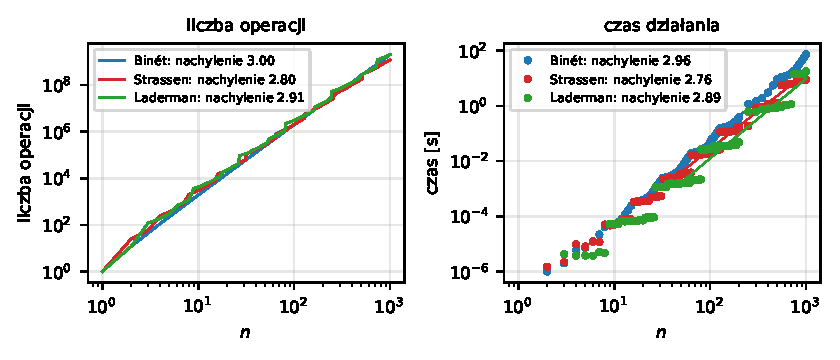
\includegraphics[width=0.86\textwidth]{data_mateusz/fig_loglog.pdf}
\caption{Wykresy w skali log-log; nachylenie dopasowanej prostej oznacza wykładnik $\alpha$ w zależności $\sim n^{\alpha}$.}
\label{fig:loglog}
\end{figure}

\section{Przykład $4\times4$ -- porównanie z Octave/MATLAB}
Do porównania wybrano $A=\texttt{magic(4)}$, $B=A^{T}/7$ (te same macierze są zaszyte w trybie
\texttt{--example} wszystkich programów). U Ladermana $n=4$ daje jedno obieranie ($r=1$) i jeden krok
właściwego algorytmu na rdzeniu $3\times3$. Skrypt \texttt{compare.m} wczytuje wyniki programów C++ i porównuje je z $A*B$
w Octave/MATLAB. Wynik referencyjny:
\[
C_{\mathrm{ref}} = A B \approx
\begin{pmatrix}
62{,}5714 & 33{,}7143 & 47{,}4286 & 21{,}4286\\
33{,}7143 & 44{,}2857 & 39{,}7143 & 47{,}4286\\
47{,}4286 & 39{,}7143 & 44{,}2857 & 33{,}7143\\
21{,}4286 & 47{,}4286 & 33{,}7143 & 62{,}5714
\end{pmatrix}.
\]
\begin{center}
\begin{tabular}{lcc}
\toprule
metoda & liczba operacji & $\max|C-C_{\mathrm{ref}}|$ \\
\midrule
Binét & 112 $(=2\cdot4^3-4^2)$ & $7{,}1\cdot10^{-15}$ \\
Strassen & 247 $(=7\cdot7^2-6\cdot4^2)$ & $1{,}4\cdot10^{-14}$ \\
Laderman & 188 $(=121+67)$ & $7{,}1\cdot10^{-15}$ \\
\bottomrule
\end{tabular}
\end{center}
Wszystkie metody dają wynik zgodny z mnożeniem wbudowanym z dokładnością do błędów zaokrągleń (rzędu $10^{-14}$);
Strassen ma nieco większy błąd, bo wykonuje więcej dodawań/odejmowań w innej kolejności. U Ladermana 121 operacji
($=8\cdot23-7\cdot9$) przypada na rdzeń $3\times3$, a 67 na cienkie iloczyny przy obieraniu.
% UWAGA: wartości referencyjne w tej wersji wyznaczono równoważnym wywołaniem A @ B w NumPy.
% Po uruchomieniu compare.m w Octave/MATLAB (dataDir = 'data_mateusz'; compare) sprawdź, czy błędy w tabeli się zgadzają.

\end{document}
